\documentclass{aa}

\usepackage{graphicx}
\usepackage{amsmath,amssymb,bm}
\usepackage{booktabs}
\usepackage{placeins}
\usepackage{tikz}
\usetikzlibrary{arrows.meta,positioning,calc}

% Inline-math spacing: if a line holding tall inline math (fractions, integrals, hats with
% sub/superscripts) would come closer than \lineskiplimit to its neighbour, TeX opens the gap to \lineskip.
% \mathsurround adds a little air on both sides of every inline formula.
\setlength{\lineskiplimit}{2pt}
\setlength{\lineskip}{3pt}
\setlength{\mathsurround}{0.6pt}

\newcommand{\mh}{[\mathrm{M}/\mathrm{H}]}
\newcommand{\msun}{M_{\odot}}
\newcommand{\kmsau}{\mathrm{km}\,\mathrm{s}^{-1}\sqrt{\mathrm{AU}}}
\newcommand{\dd}{\,\mathrm{d}}
\newcommand{\Normal}{\mathcal{N}}
\newcommand{\StudentT}{\mathcal{T}}
\newcommand{\indicator}{\mathbb{I}}
\newcommand{\softplus}{\operatorname{softplus}}
\newcommand{\sigmoid}{\operatorname{sigmoid}}

\begin{document}

\title{Dynamical calibration of a metallicity-dependent stellar mass--luminosity relation from Gaia wide binaries}
\author{Yu-Ting Wang\inst{1}\email{yuwang@mpia.de}
        \and Hans-Walter Rix\inst{1}\email{rix@mpia.de}
        %\and Jiadong Li\inst{1}\corrauth{jdli@mpia.de}
        \and Jiadong Li\inst{1}\email{jdli@mpia.de}
        \and Yuan-Sen Ting\inst{2}\email{ting.74@osu.edu}
        }

\institute{Max-Planck-Institut f\"ur Astronomie, K\"onigstuhl 17, 69117 Heidelberg, Germany
          \and The Ohio State University, 140 W. 18th Ave., Columbus, OH 43210, USA}


\abstract
  {The masses of low-mass main-sequence stars are tightly related to their positions in the colour--magnitude diagram, but this relation depends on metallicity, and its empirical calibration rests on a small number of systems with dynamical masses.}
  {We calibrate the mass--luminosity relation (MLR) of main-sequence stars as a function of absolute $G$ magnitude and metallicity, using a large sample of wide binaries from Gaia with precisely measured relative positions and proper motions.}
  {We extend the statistical approach of \citet{Hwang2024DynamicalMasses} in three respects. Metallicities are taken from Gaia XP spectra (J-CaPS), with the components of each pair constrained to a common value; unresolved binaries are removed on the basis of the XP spectra; and the MLR is described by a monotone two-dimensional B-spline surface in absolute $G$ magnitude ($3.5\le M_{\mathrm{G}}\le13.5$ mag) and calibrated metallicity $Z$ ($-1.0\le Z\le0.6$\,dex). The surface is fitted with a likelihood that accounts for the measurement uncertainties, an outlier component and the selection of the sample.}
  {The MLR is tightly constrained over this range of metallicity. This statistical dynamical calibration is largely consistent with individual mass measurements from orbital motions, asteroseismology and eclipsing binaries. Both approaches indicate that PARSEC isochrones overpredict stellar masses by about $10\%$ at $M_{\mathrm{G}}>9$ mag.% TODO: add numbers: offset from Mann et al. (2019), metallicity dependence, outlier fraction.
  }
  {}

   \keywords{binaries: visual -- stars: low-mass -- stars: fundamental parameters -- methods: statistical -- Galaxy: solar neighbourhood}

\titlerunning{Dynamical calibration of the stellar MLR}
\authorrunning{Y. Wang}

\maketitle

%==============================================================================
\section{Introduction}\label{sec:intro}

In this paper, we calibrate the mass--luminosity relation (MLR) of main-sequence stars over the absolute magnitude range $3.5\le M_{\mathrm{G}}\le13.5$ mag as a function of metallicity. At solar metallicity this range corresponds to masses of about $0.1$ to $1.3\,\msun$, from late-F and G dwarfs down to the bottom of the main sequence, and our focus is on the K and M dwarfs that make up most of it.

Stars of low mass are the numerically dominant stellar population. M dwarfs make up roughly three quarters of the stars within 10\,pc of the Sun \citep{Henry2018}, and an initial mass function that is flat or declining below $\sim0.5\,\msun$ \citep{Kroupa2001,Chabrier2003} still places a large part of the stellar mass of the Galactic disk in stars below one solar mass \citep{Chabrier2001}. They therefore hold much of the baryonic mass that has been locked up in stars, and the mass function inferred from star counts, and every quantity derived from it (the mass-to-light ratio of stellar populations, the contribution of dwarfs to the dynamical mass budget of the disk, the claimed variations of the IMF with environment and metallicity), depends directly on how masses are assigned to dwarfs. The assignment is not innocuous: a mass--luminosity relation that is wrong in one photometric band propagates into the local mass function derived from the luminosity function in that band \citep{Delfosse2000}. Low-mass stars are also the most common hosts of small planets \citep{Dressing2015}. The radius of a transiting planet scales with the stellar radius, which for a dwarf is obtained from its mass or luminosity \citep{Mann2015}, the semi-amplitude of its radial-velocity signal scales as $M_\star^{-2/3}$, and the distance of the habitable zone depends on the stellar luminosity and thus again on mass. Errors of a few per cent in the stellar mass pass into the planetary mass, radius and bulk density.

Stellar mass is almost never a measured quantity. Asteroseismology provides an independent route for single stars: the frequency of maximum power and the large frequency separation of solar-like oscillations give the mass and radius of a star without a companion, and have been applied to thousands of red giants and to hundreds of dwarfs and subgiants \citep{ChaplinMiglio2013,Serenelli2017,Pinsonneault2018}. The oscillation amplitude decreases steeply towards lower luminosity \citep{Kjeldsen1995}, so the detections are concentrated in giants and in dwarfs hotter than about 5000\,K, and K and M dwarfs are essentially out of reach \citep{ChaplinMiglio2013}. The giants, which are the bulk of the asteroseismic sample, are evolved and cannot calibrate a main-sequence MLR.

Binaries are therefore the main place where stellar masses are calibrated, and the methods differ in what they measure. In eclipsing binaries with double-lined spectroscopic orbits, the radial-velocity amplitudes and the orbital inclination from the eclipse light curve give the mass of each component directly, to a few per cent or better \citep{Torres2010}. The systems are, however, close, with periods of days, so tidal interaction and fast rotation may alter the stars, and low-mass eclipsing binaries are among those that show the radius and temperature anomalies discussed below. 

Visual and astrometric orbits of nearby binaries determine the total mass from Kepler's third law once the period, the semi-major axis and the parallax are known, and the mass ratio from the motion of the components about the barycentre. Combined with long-term imaging and adaptive optics this is the basis of the best relations for M dwarfs \citep{Henry1993,Delfosse2000,Benedict2016,Mann2019}. It needs monitoring over years to decades, requires systems that are close enough to be resolved, and has produced samples of a few tens of systems. 

Spectroscopic binaries without eclipses give the projected orbit only. For double-lined systems (SBII) the radial velocities of both stars yield $M\sin^3 i$ for each component, and for single-lined systems (SBI) only the mass function, a combination of the two masses and the inclination that cannot be inverted without an assumption on the mass of the visible star. In both cases the inclination is unknown, unless it is supplied by an astrometric orbit. The Gaia astrometric and spectroscopic orbits \citep{GaiaCollaboration2023NSS} make such combinations possible for large numbers of binaries and have been used to derive the MLR in the $G$ band down to $0.12\,\msun$ \citep{Chevalier2023}, but the solutions are restricted to periods of the order of the mission length and to systems with a resolvable photocentre motion, and the SBI solutions depend on an adopted mass of the primary.

For all other stars the mass has to be inferred from an observable that correlates with it, usually the absolute magnitude, through a calibrated MLR, and because the calibrating systems are rare, the empirical relations rest on a few tens of systems. The near-infrared relation of \citet{Mann2019}, the most precise, is based on 62 binaries and yields masses to $2$--$3\%$. It finds no measurable dependence on metallicity at the solar-neighbourhood level, but this holds for the $K_s$ band and for a narrow metallicity range, and the dependence in bands that are more sensitive to molecular absorption, such as the optical bands of Gaia, is not constrained in the same way.

%For the large photometric samples of Gaia the relation is usually taken from stellar evolution models, whose predictions for low-mass stars remain uncertain. The interior structure depends on the treatment of convection, for which mixing-length theory has to be calibrated or replaced by fits to multidimensional simulations, and on the equation of state and opacities at high density \citep{ChabrierBaraffe2000,Baraffe2015}. The emergent flux, and hence the colours and bolometric corrections that connect a model luminosity to a Gaia magnitude, are governed by molecular opacities (TiO, VO, H$_2$O) whose line lists are incomplete, so that models have long predicted optical colours that disagree with observed M dwarfs \citep{Baraffe2015}. The \textsc{PARSEC} models required an empirical shift of the temperature--optical-depth relation of the atmosphere, calibrated on the observed mass--radius relation, to reproduce the lower main sequence \citep{Chen2014}. Eclipsing binaries show in addition that low-mass stars have radii larger and effective temperatures lower than predicted by non-magnetic models at the same mass, a discrepancy that is attributed to magnetic activity and spots but is not yet fully explained \citep{TorresRibas2002,FeidenChaboyer2012,Spada2013,FeidenChaboyer2014}. These effects change both the luminosity and the colour at fixed mass, and the effect on the MLR depends on band and on metallicity, because metallicity controls the opacity of the atmosphere and the interior. The discrepancy between models and observations is largest in the visual bands and decreases in the near-infrared \citep{Delfosse2000}. A calibration in the Gaia bands as a function of metallicity, which can be compared with model predictions, is therefore missing.

Wide binaries offer a way to obtain such a calibration for large samples. Their projected separations are $10^3$--$10^4$\,au and their orbital periods $10^4$--$10^6$\,yr, so no orbit can be followed, and each pair provides a single snapshot: the projected separation $s$ and the plane-of-sky velocity difference $\Delta v$ of the two components. Kepler's law nevertheless relates these quantities to the total mass, $\Delta v\sqrt{s}\propto\sqrt{M_{\rm tot}}$, with a proportionality that depends on the orbital phase, eccentricity and inclination of the pair. For a population with random phases, orientations and a known eccentricity distribution, the distribution of $u=\Delta v\sqrt{s}$ has a fixed shape whose scale is set by the mass, so the mass of a group of pairs can be recovered statistically. Gaia has made this practical: its astrometry gives the proper-motion difference and the parallax of hundreds of thousands of pairs \citep{ElBadry2021MillionBinaries}. The same relative velocities have been used to test gravity at the low accelerations of wide pairs, where the stellar masses are taken from a relation and the shape of the distribution of $\Delta v$ is compared with Newtonian and modified-gravity predictions \citep{Hernandez2012,Chae2023,Banik2024}. The inverse problem, in which Newtonian dynamics is assumed and the mass is inferred, has been applied to calibrate an MLR in the $G_{\rm RP}$ band with a few thousand pairs \citep{Giovinazzi2022}. 

\citet{Hwang2024DynamicalMasses} extended this idea to the whole Hertzsprung--Russell diagram. 
%Using the wide binaries of the \citet{ElBadry2021MillionBinaries} catalogue, they modelled the mass of a star as a neural-network function of its colour and absolute magnitude and trained it by maximising the likelihood of $u$, with a mixture component for high-$u$ outliers. The resulting map from position in the diagram to stellar mass relies only on Newtonian dynamics, covers main-sequence stars from $0.1$ to $2\,\msun$ as well as pre-main-sequence stars, unresolved multiples, giants and white dwarfs, and shows that Gaia wide binaries provide a model-independent mass scale of broad applicability. 
It has, however, three limitations for a calibration of the single-star MLR. First, the map gives the mean mass of whatever population occupies a position in the diagram (single stars, unresolved binaries and triples, pre-main-sequence stars overlap on the lower main sequence), so the single-star relation is read off a running median. Second, the input has no metallicity, which the authors identify as a natural extension. Third, the uncertainty is the scatter of repeated network predictions with dropout, not a posterior that includes the measurement errors, the outlier model and the sample selection; in particular, the cut on the significance of the proper-motion difference is satisfied through distance and separation limits but not modelled in the likelihood.

Here we build on this approach and turn it into a calibration of the MLR of single main-sequence stars. We use the pairs of the \citet{ElBadry2021MillionBinaries} catalogue for which J-CaPS metallicities \citep{Li2026JCaPS} are available for both components. Gaia BP/RP spectra allow us to identify and remove unresolved binaries, so that the sample consists almost entirely of true wide pairs of single main-sequence stars and the relation refers to a well-defined population rather than to the mean of all stars at a position in the diagram. Metallicity is a variable of the model, and we fit a monotone MLR surface in absolute $G$ magnitude and metallicity. The likelihood for $u$ includes the measurement errors, an outlier component, and the truncation produced by the catalogue's cut on the significance of the proper-motion difference.

The paper is organised as follows. Section~\ref{sec:data} describes the data, Sect.~\ref{sec:method} the inference, Sect.~\ref{sec:results} the resulting MLR, and Sect.~\ref{sec:systematics} the tests of the main modelling assumptions. We discuss the results and their limitations in Sect.~\ref{sec:discussion} and conclude in Sect.~\ref{sec:conclusions}.

%==============================================================================
\section{Data}\label{sec:data}
\subsection{Wide-binary catalogue}
Our sample is drawn from the catalogue of \citet{ElBadry2021MillionBinaries}, who searched Gaia EDR3 for resolved pairs of stars within about 1\,kpc of the Sun whose parallaxes and proper motions are consistent with a gravitationally bound orbit, and obtained about $1.3\times10^6$ candidate wide binaries with projected separations from a few au up to 1\,pc. The catalogue was not built from a catalogue of known binaries, and its contamination by chance alignments was estimated empirically from the density of pairs found in a sample with shifted positions. Each pair carries the quantity \texttt{R\_chance\_align}, an estimate of the probability that it is a chance alignment, which we use below to remove most of the contaminants. We apply further quality cuts to ensure reliable astrometry and photometry.

We require $\texttt{R\_chance\_align}<0.1$ and $s<10^4~\mathrm{AU}$ to eliminate most chance alignments, $\varpi>1~\mathrm{mas}$, $\texttt{Fidelity\_v2}\geq 0.5$ to ensure stars with reliable astrometry. We further require Gaia flux signal-to-noise ratios $>10$, $|C^\ast|\leq 3\sigma_{C^\ast}$ to remove sources with poor BP/RP observations, a blended-transit fraction $\beta>0.5$ to remove sources affected by blending.

\begin{table*}[ht]
\centering
\caption{Quality cuts applied to the wide binaries of the \citet{ElBadry2021MillionBinaries} catalogue.}
\label{tab:quality_cuts}
\begin{tabular}{@{}lcl@{}}
\toprule
Criterion & Cut & Purpose \\
\midrule
$\texttt{R\_chance\_align}$ & $<0.1$ & Eliminate chance alignments \\
$s$ (projected separation) & $<10^4~\mathrm{AU}$ & Eliminate chance alignments \\
$\varpi$ (parallax) & $>1~\mathrm{mas}$ & Targeted distance volume \\
$\texttt{Fidelity\_v2}$ & $\geq 0.5$ & Stars with reliable astrometry \\
$\Delta\mathrm{BIC}$ & $>0$ & XP-based single-star classification, both components (Sect.~\ref{sec:jcaps}) \\
J-CaPS quality cuts & \textbf{TODO} & \textbf{TODO} \\
Gaia flux S/N & $>10$ & High-quality photometry \\
$|C^\ast|$ & $\leq 3\sigma_{C^\ast}$ & Good BP/RP observations \\
$\beta$ (blended-transit fraction) & $>0.5$ & Remove blended sources \\
$u/\sigma_u$ (relative-velocity S/N) & $>3$ & Reliable velocity measurements \\
\bottomrule
\end{tabular}
% TODO: cite sources of Fidelity_v2, C^*, beta (cf. Rybizki, Riello) once the references are fixed.
\end{table*}

\subsection{J-CaPS metallicities and the single-star criterion}\label{sec:jcaps}
The metallicities come from J-CaPS \citep{Li2026JCaPS}, a JAX-based code that fits Gaia DR3 BP/RP (XP) spectra with a neural-network forward model of effective temperature, absolute magnitude $M_{\mathrm{G}}$ and metallicity $[\mathrm{M/H}]_{\rm JC}$, in the spirit of The Payne. The network is trained on about $7.7\times10^4$ single stars whose reference labels are the calibrated ASPCAP parameters of SDSS-V/APOGEE, and a new spectrum is fitted by minimising the $\chi^2$ between the observed and the model spectrum, starting from an initial guess from a multilayer perceptron. Its typical metallicity uncertainty is $\sim0.25$\,dex at $[\mathrm{M/H}]_{\rm JC}<-1$, and the training set is sparse at low metallicity and low mass, with ASPCAP temperatures that may be offset for red dwarfs below $4500$\,K. We use the raw J-CaPS metallicity of each component and its reported uncertainty as $\widehat z_{jk}$ and $\sigma_{z,jk}$ (Sect.~\ref{sec:overview}), and correct for their systematics through a magnitude-dependent relative bias $b_G$ that Stage~1a fits from the differences within binaries and a zero-point offset $\delta_z$ set by a solar anchor in Stage~1b (Sect.~\ref{sec:stage1}). We also apply quality cuts to the J-CaPS measurements before they are used: \textbf{[TODO: J-CaPS quality cuts (quantities, thresholds and purpose), to be supplied.]}

The single-star criterion is taken from the analysis of Gaia XP spectra of \citet{Li2025BinaryXP}, who fit each spectrum with a single-star model and with a binary model that adds a companion described by its mass ratio. The $\chi^2$ of the two fits define the criterion. We compare the models through the Bayesian information criterion, which penalises the additional parameters of the binary model,
\begin{equation}
 \mathrm{BIC}=\chi^2+k\ln n,
 \label{eq:bic}
\end{equation}
and define
\begin{equation}
 \Delta\mathrm{BIC}=\mathrm{BIC}_{\rm binary}-\mathrm{BIC}_{\rm single}.
 \label{eq:dbic}
\end{equation}
A positive $\Delta\mathrm{BIC}$ means that the single-star model describes the spectrum at least as well as the binary model once its smaller number of parameters is accounted for, and we require $\Delta\mathrm{BIC}>0$ for both components of a wide binary, so that a pair is kept only if both stars are single. This removes unresolved binaries, whose composite spectra would otherwise bias both the metallicity and the mass--luminosity relation, and leaves a sample of single main-sequence stars.
% TODO: k and n used in the BIC.

\subsection{Observed relative velocity}
% Definition of $u=\Delta v_{\rm tan}\sqrt{r_\perp}$ and $\sigma_u$; distribution of $u$ and $\sigma_u$ in the sample.
% Figure: sample in CMD coloured by metallicity; $u$ vs separation.

We calculate $u$ for each wide binary system of the \citet{ElBadry2021MillionBinaries} catalogue from Gaia DR3 observables. For a pair with parallax $\varpi$, angular separation $\theta$ and proper-motion difference $\Delta\mu$ between its two components, the projected separation and the plane-of-sky relative speed are
\begin{equation}
 s=\frac{\theta}{\varpi},\qquad v=k\,\frac{\Delta\mu}{\varpi},
 \label{eq:sv}
\end{equation}
where $\Delta\mu/\varpi$ is the relative velocity in $\mathrm{au\,yr^{-1}}$ for $\Delta\mu$ and $\varpi$ in the same angular unit, $k=4.74\,\mathrm{km\,s^{-1}}\,\mathrm{yr\,au^{-1}}$ converts it to $\mathrm{km\,s^{-1}}$, and $s$ is in au for $\theta$ and $\varpi$ in arcsec. The statistic of Eq.~(\ref{eq:u}) is then
\begin{equation}
 u=v\sqrt{s}\quad[\kmsau].
 \label{eq:uobs}
\end{equation}
The velocity difference in the plane of the sky has independent Gaussian errors of the same scale $\sigma_{u,j}$ on both components, so $u_j$ is the magnitude of a two-dimensional Gaussian vector and follows a Rice distribution (Sect.~\ref{sec:dynamics}). The scale is obtained from the significance of the proper-motion difference,
\begin{equation}
 \sigma_{u,j}=\frac{u_j}{(\Delta\mu/\sigma_{\Delta\mu})_j},
 \label{eq:sigu}
\end{equation}
so that the requirement $u/\sigma_u>3$ of Table~\ref{tab:quality_cuts} is the same as the requirement that $\Delta\mu$ is detected at more than $3\sigma$. Since $\sigma_{u,j}$ is fixed for each pair by the catalogue astrometry, this cut acts as a threshold on the observed statistic, and we model it in the likelihood (Sect.~\ref{sec:selection}).

The overall selection criteria are summarised in Table~\ref{tab:quality_cuts}.
% TODO: check that the pair parallax and the angular separation are taken as in the catalogue (parallax of the primary or mean of the two components), and that sigma_Delta_mu includes the full astrometric covariance.
% TODO: add the distributions of u, sigma_u and s in the final sample, and the figures listed above.

%==============================================================================
\section{Method}\label{sec:method}
\subsection{Overview}\label{sec:overview}
The inference is modular. Stage~1a uses the metallicity differences between the two components of each binary to estimate the relative calibration of the J-CaPS metallicities. Conditional on this estimate, Stage~1b combines the J-CaPS measurements of both components with a hierarchical population distribution of metallicities, and returns a posterior probability distribution for the shared metallicity $Z_j$ of every binary. Stage~2 takes these distributions as fixed inputs, predicts the masses of both components from a metallicity-dependent MLR at every metallicity, and evaluates the wide-binary dynamical likelihood, corrected for the selection of the sample by the significance of the proper-motion difference. The workflow is shown in Fig.~\ref{fig:workflow}.

\begin{figure*}[t]
\centering
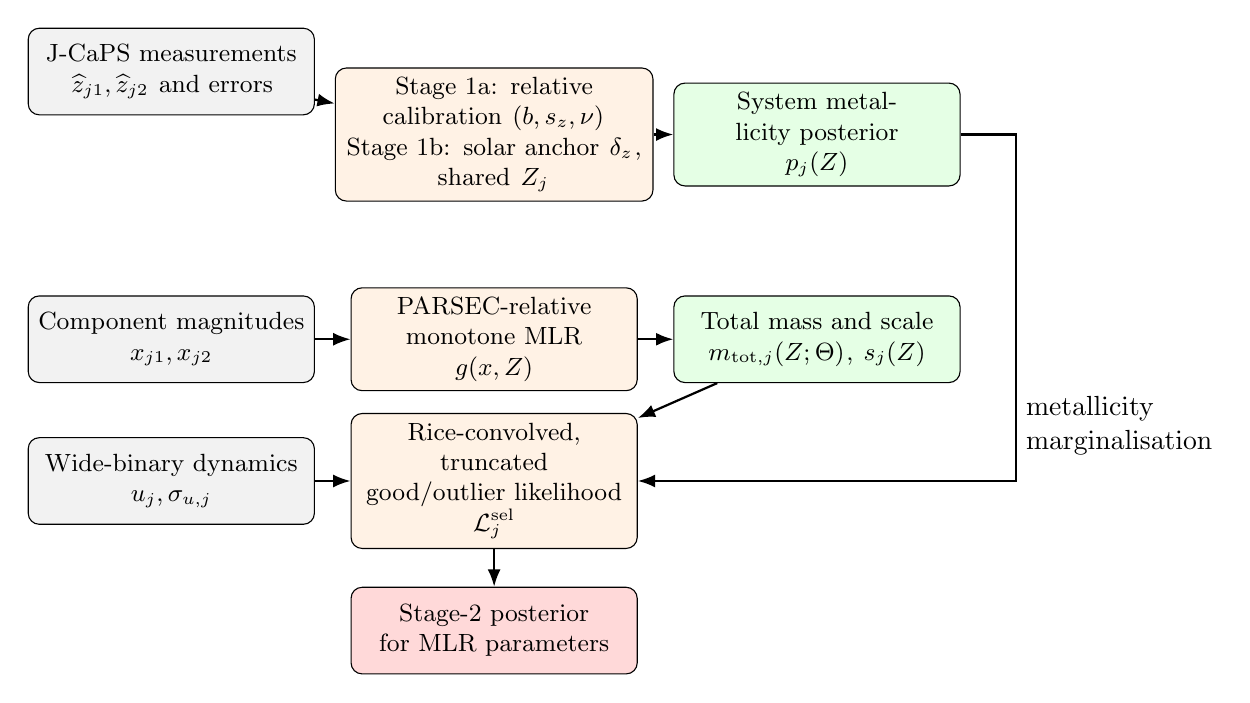
\begin{tikzpicture}[
  box/.style={draw,rounded corners,align=center,minimum height=11mm,text width=34mm,fill=blue!5,font=\small},
  data/.style={box,fill=gray!10},
  model/.style={box,fill=orange!10},
  result/.style={box,fill=green!10},
  end/.style={box,fill=red!15},
  arrow/.style={-{Latex[length=2.2mm]},thick}
]
\node[data]   (spec)   at (0, 2.6) {J-CaPS measurements\\$\widehat z_{j1},\widehat z_{j2}$ and errors};
\node[model,text width=38mm]  (stage1) at (4.1, 1.8) {\small Stage 1a: relative calibration $(b,s_z,\nu)$\\Stage 1b: solar anchor $\delta_z$,\\shared $Z_j$};
\node[result] (weights)at (8.2, 1.8) {System metallicity posterior\\$p_j(Z)$};
\node[data]   (phot)   at (0,-0.8) {Component magnitudes\\$x_{j1},x_{j2}$};
\node[model]  (mlr)    at (4.1,-0.8) {PARSEC-relative\\monotone MLR\\$g(x,Z)$};
\node[result] (mass)   at (8.2,-0.8) {Total mass and scale\\$m_{{\rm tot},j}(Z;\Theta)$, $s_j(Z)$};
\node[data]   (dyn)    at (0,-2.6) {Wide-binary dynamics\\$u_j,\sigma_{u,j}$};
\node[model]  (rice)   at (4.1,-2.6) {Rice-convolved, truncated\\good/outlier likelihood\\$\mathcal L^{\rm sel}_j$};
\node[end]    (post)   at (4.1,-4.5) {Stage-2 posterior\\for MLR parameters};
\draw[arrow] (spec) -- (stage1);
\draw[arrow] (stage1) -- (weights);
\draw[arrow] (phot) -- (mlr);
\draw[arrow] (mlr) -- (mass);
\draw[arrow] (mass) -- (rice);
\draw[arrow] (dyn) -- (rice);
\draw[arrow] (rice) -- (post);
\draw[arrow] (weights.east) -- ++(7mm,0) |- node[pos=0.42,right,align=left]{metallicity\\marginalisation} (rice.east);
\end{tikzpicture}
\caption{Inference workflow. Stage~1a estimates the relative J-CaPS calibration from within-binary differences. Conditional on these estimates, Stage~1b returns a posterior distribution of the shared metallicity of each system. Stage~2 propagates this uncertainty into the dynamical MLR fit but does not update either Stage~1 module.}
\label{fig:workflow}
\end{figure*}

In the following description, binary systems are indexed by $j$, their components by $k\in\{1,2\}$. Hats denote observed quantities. $x_{jk}$ is the Gaia absolute magnitude $M_{\mathrm{G}}$ of a component, $\widehat z_{jk}\equiv[\mathrm{M/H}]_{{\rm JC},jk}$ the raw J-CaPS metallicity and $\sigma_{z,jk}$ its reported error. We write $Z$ (in dex) for the calibrated metallicity, that is, the metallicity on the PARSEC $[\mathrm{M/H}]$ scale after the corrections of Sect.~\ref{sec:stage1}, and $Z_j$ for that of system $j$. The MLR and all results below are functions of $Z$, not of $[\mathrm{M/H}]_{\rm JC}$. 

\subsection{System metallicities}\label{sec:stage1}
\paragraph{Relative calibration (Stage~1a).} The J-CaPS metallicity of a star may be biased, and the bias may depend on the magnitude of the star. We model each measurement as an independent Student-$t$ draw around the shared metallicity of the pair,
\begin{equation}
 \widehat z_{jk}\mid Z_j \sim \StudentT_{\nu}\!\left[Z_j+\delta_z+b\cdot x_{jk},\ \sqrt{\sigma_{z,jk}^2+s_z^2}\right]\equiv\mathcal L^{\rm spec}_{jk}(Z_j),
 \label{eq:spec-model}
\end{equation}
where $\delta_z$ is the zero-point offset of J-CaPS with respect to the true metallicity scale at the reference magnitude $x_{\rm ref}$, $b_G(x)=b\,(x-x_{\rm ref})$ is a bias that varies linearly with absolute magnitude with slope $b$, $s_z$ is an additional scatter common to all stars, and $\nu$ the degrees of freedom. Conditional on $Z_j$ the two components are independent. The two stars of a wide binary share the same metallicity, so the difference of their measurements removes $Z_j$ and $\delta_z$,
\begin{equation}
 \widehat z_{j1}-\widehat z_{j2}\sim\StudentT_{\nu}\!\left[b\,(x_{j1}-x_{j2}),\ \sqrt{\sigma_{z,j1}^2+\sigma_{z,j2}^2+2s_z^2}\right],
 \label{eq:zdiff}
\end{equation}
and depends only on the relative parameters. Stage~1a therefore corrects the \emph{relative} systematics of J-CaPS: the slope $b$ of the bias with the magnitude difference, the extra scatter $s_z$ and the degrees of freedom $\nu$ are fitted to the observed metallicity differences by maximum likelihood and are held fixed in Stage~1b. These differences are blind to a common offset.

\paragraph{Absolute calibration and system posteriors (Stage~1b).} The common offset $\delta_z$, which sets the absolute metallicity scale, requires external anchors, that is, stars whose true metallicity is known, and one or more of them can be used. We use a single solar anchor: we take the J-CaPS metallicity of a star with the absolute magnitude of the Sun, $M_{\mathrm{G},\odot}\approx4.67$, to be unbiased and set $x_{\rm ref}=M_{\mathrm{G},\odot}$ and $Z_{\mathrm{ref}}=0$, so that $\delta_z+b\cdot x_{\rm ref}=0$.

%The metallicity is evaluated on a grid of $81$ nodes $Z_q$ between $-1.0$ and $0.6$\,dex. The population distribution is a mixture of six truncated Gaussians with equally spaced centres on this interval, a common width equal to the interval divided by six, and weights $\bm\omega$ with a flat Dirichlet prior. With $\delta_z$ fixed by the anchor, the weights $\bm\omega$ are the only global parameters, and the unnormalised density of one system is
% \begin{equation}
%  \widetilde p_j(Z,\bm\omega)=p_{\rm pop}(Z\mid\bm\omega)\,p(\bm\omega)\prod_{k=1}^{2}\mathcal L^{\rm spec}_{jk}(Z),
%  \label{eq:zpost}
% \end{equation}
% and $\bm\omega$ is inferred from the product of the marginal evidences of all systems. The posterior probability mass of system $j$ at node $Z_q$, with $\bm\omega$ fixed at its posterior mean, is $\overline P_{jq}$. This single distribution per system is the only metallicity information passed to Stage~2.

We plot the colour-magnitude diagrams of the final sample in Fig.~\ref{fig:cmd}, binned by the median metallicity of each system.

\begin{figure*}[t]
\centering
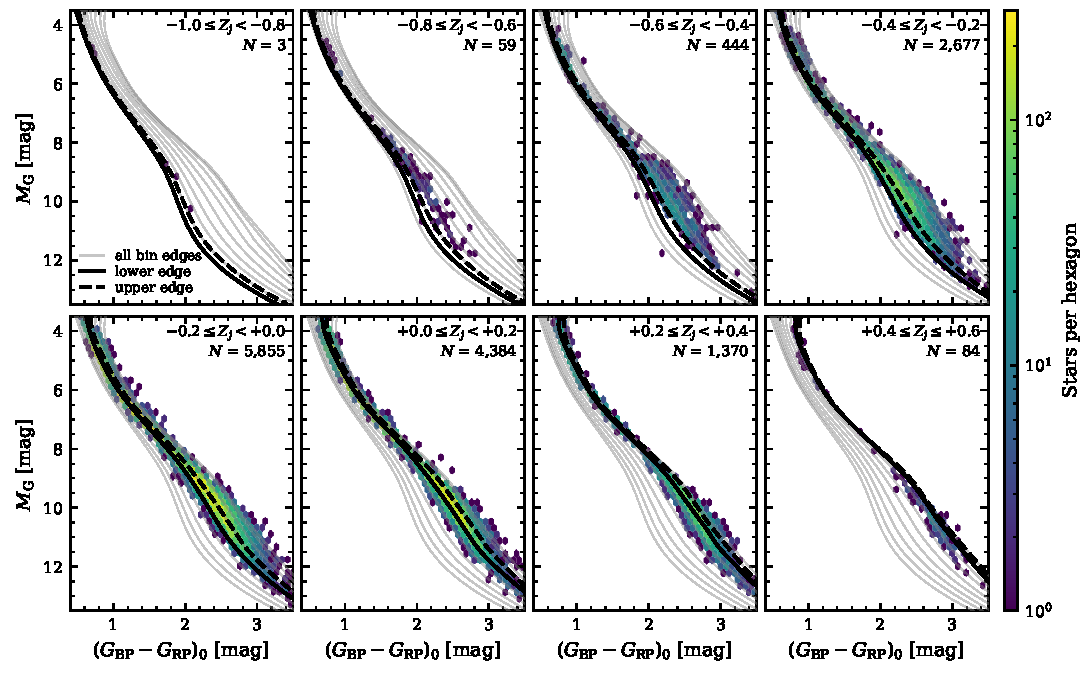
\includegraphics[width=\textwidth]{figs/cmd_by_zj_bin.pdf}
\caption{Colour--magnitude diagrams of the components of the selected wide binaries, in bins of the posterior median of the system metallicity $Z_j$ (Stage~1b). The colour scale shows the number of stars per hexagon, and the number of stars in each bin is given in the panels. The black solid and dashed lines are the PARSEC main sequences at the lower and upper edge of the bin of each panel, and the grey lines are those at all bin edges, repeated in every panel for reference.}
% TODO: state which PARSEC age range the plotted colour--magnitude relation averages over.
\label{fig:cmd}
\end{figure*}


\subsection{MLR parameterisation: a 2-D B-spline surface}\label{sec:mlr}
We describe the mass of a star of absolute magnitude $x$ and metallicity $Z$ by the surface $g(x,Z)=\log_{10}[M/\msun]$. The surface is a tensor-product cubic B-spline \citep{deBoor2001Splines} with $8$ coefficients in $x$ and $4$ in $Z$,
\begin{equation}
 g(x,Z)=\sum_{i=1}^{8}\sum_{h=1}^{4}\Theta_{ih}B_i(x)C_h(Z),
 \label{eq:g-total}
\end{equation}
with clamped knots at
\begin{align}
 x&=\{3.5,5.5,7.5,9.5,11.5,13.5\}\,\mathrm{mag},\\
 Z&=\{-1.0,0.6\}\,\mathrm{dex}.
 \label{eq:knots}
\end{align}
The coefficients are written $\Theta=\Pi+D$, where $\Pi$ is the projection of the PARSEC mass surface $g_{\rm P}(x,Z)$ onto the same basis and $D$ is the correction relative to PARSEC MLRs fitted to the data. The mass relation is then reported relative to PARSEC through $\Delta_{\rm P}=g-g_{\rm P}$, which includes the small projection error (RMS $0.002$\,dex). We impose two physical constraints: a fainter star at fixed metallicity is not more massive, and a more metal-rich star at fixed magnitude is not less massive,
\begin{equation}
 \Theta_{i+1,h}\le\Theta_{ih},\qquad \Theta_{i,h+1}\ge\Theta_{ih}.
 \label{eq:coefficient-order}
\end{equation}
These inequalities on the B-spline coefficients imply $\partial g/\partial x\le0$ and $\partial g/\partial Z\ge0$ everywhere in the domain. They apply to the total surface and not to $D$, so the correction itself may have either sign and the data are free to move the relation away from PARSEC. No constraint is placed on the mixed differences. The inequalities are enforced by construction through a reparametrisation with unconstrained variables (see Appendix~\ref{app:model}).

\subsection{Dynamical likelihood}\label{sec:dynamics}
\paragraph{Mass-scaled velocity statistic.} In a bound binary, the total mass $m_{\rm tot}=m_1+m_2$, the semi-major axis $a$, the eccentricity $e$ and the orbital phase set the instantaneous relative speed,
\begin{equation}
 v_{\rm rel}=\sqrt{\frac{Gm_{\rm tot}}{a}}\,f(\theta,e),
\end{equation}
where $f(\theta,e)$ describes the variation along the ellipse, from $f=\sqrt{(1+e)/(1-e)}$ at pericentre to $f=\sqrt{(1-e)/(1+e)}$ at apocentre. We observe only the projected speed $v$ and the projected separation $s$, and use the statistic
\begin{equation}
 u=v\sqrt{s}.
 \label{eq:u}
\end{equation}
Because $v\propto a^{-1/2}$ and $s\propto a$, the semi-major axis cancels, and $u\propto\sqrt{m_{\rm tot}/\msun}$ with a factor that depends only on the eccentricity, the phase and the orientation of the orbit. Dividing out the mass, $\widetilde u=u/\sqrt{m_{\rm tot}/\msun}$ depends only on these nuisance parameters, which we marginalise once in a simulation of orbits to obtain a distribution $p(\widetilde u)$ that does not depend on mass (see below). A noiseless measurement then has the density
\begin{equation}
 p(u\mid m_{\rm tot})=\frac{1}{\sqrt{m_{\rm tot}/\msun}}\,p\!\left(\frac{u}{\sqrt{m_{\rm tot}/\msun}}\right).
\end{equation}

\paragraph{From the MLR to the likelihood of a pair.} The quantity we want to constrain is the relation $g(x,Z)$ between absolute magnitude, metallicity and mass (Sect.~\ref{sec:mlr}). The mass of a component of absolute magnitude $x_{jk}$ in a system of metallicity $Z$ is $m_{jk}(Z)=\msun10^{g(x_{jk},Z;\Theta)}$, so that the total mass of pair $j$ is
\begin{equation}
 m_{{\rm tot},j}(Z;\Theta)=m_{j1}(Z)+m_{j2}(Z),
\end{equation}
and the mass scale entering $p(u\mid m_{\rm tot})$ is $s_j(Z)=\sqrt{m_{{\rm tot},j}(Z)/\msun}$. The parameters $\Theta$ of the MLR therefore enter the dynamical likelihood only through the total masses of the pairs, and the metallicity $Z$ of each system is a nuisance parameter that is marginalised over its Stage-1b posterior (Sect.~\ref{sec:selection}).

\paragraph{Measurement errors.} The uncertainty of $u$ comes mainly from the uncertainty $\sigma_{\Delta\mu}$ of the proper-motion difference. The observed $\Delta\mu$ is the magnitude of a two-dimensional vector with Gaussian errors, and therefore follows a Rice distribution \citep{Rice1945}. At fixed distance and separation $u\propto\Delta\mu$, so the observed $u_j$ follows the same distribution, given the noiseless value $v$ of $u$ and the scale $\sigma_{u,j}$,
\begin{equation}
 R(u_j\mid v,\sigma_{u,j})=\frac{u_j}{\sigma_{u,j}^2}\exp\!\left[-\frac{u_j^2+v^2}{2\sigma_{u,j}^2}\right]I_0\!\left(\frac{u_jv}{\sigma_{u,j}^2}\right),
 \label{eq:rice}
\end{equation}
where $I_0$ is the modified Bessel function of order zero and $\sigma_{u,j}=u_j/(\Delta\mu/\sigma_{\Delta\mu})_j$ (Sect.~\ref{sec:data}). The likelihood of a bound pair with mass scale $s$ is the convolution of $p(\widetilde u)$ with this measurement kernel.

\paragraph{Good and outlier components.} Not all pairs in the sample are bound binaries of two single stars: some contain an unresolved third body, and a few may be chance alignments. For these the relation between $u$ and the mass of the two components does not hold. We therefore describe each pair by a mixture of a good component, whose mass scale is that of the two stars, and an outlier component that does not depend on mass,
\begin{multline}
 \mathcal L_j(s)=(1-f_{\rm outlier})\int_0^{\infty}p(\widetilde u)\,R(u_j\mid s\widetilde u,\sigma_{u,j})\dd\widetilde u\\+f_{\rm outlier}\int_0^{\infty}q(v)\,R(u_j\mid v,\sigma_{u,j})\dd v,
 \label{eq:mixture}
\end{multline}
where the first integral carries the Jacobian $1/s$ of the change of variable from $v$ to $\widetilde u$ and the outlier fraction $f_{\rm outlier}$ is a free parameter. Here, $p(\widetilde u)$ and $q(v)$ are the distributions of the good and the outlier component, in units of $\kmsau$.

\paragraph{Shape of the good component.} The good component uses the functional form of \citet{Hwang2024DynamicalMasses},
\begin{equation}
 p(\widetilde u)=\frac{1}{N}\,\widetilde u\exp\!\left[-B\widetilde u^2-\exp\!\left(\frac{\widetilde u-u_c}{C}\right)\right],
 \label{eq:good}
\end{equation}
with re-calibrated parameters $B=2.5050\times10^{-3}$, $u_c=37.2461$ and $C=2.4500$, and $N$ normalising $p$ on $(0,\infty)$. The constants are fitted to a Monte Carlo of Keplerian orbits with uniform mean anomalies, isotropic orientations and eccentricities drawn from $p(e)\propto e^{\alpha_e}$, in which each simulated pair is weighted so that its joint distribution of projected separation and distance matches the sample (see Appendix~\ref{app:pu} for more details). We adopt $\alpha_e=1.23$, the separation-dependent power-law index of \citet{Hwang2022Eccentricity} evaluated at the projected separations of our pairs. That index is measured from the angle between the separation and relative-velocity vectors of Gaia wide binaries and does not involve stellar masses. The shape is held fixed, and the effect of $\alpha_e$ on the MLR is quantified in Sect.~\ref{sec:sys_pu}. Its upper edge is set by energy conservation, $\widetilde u<\sqrt{2G\msun/\mathrm{AU}}=42.12\,\kmsau$ for any eccentricity distribution.

\paragraph{Shape of the outlier component.} The outlier component is a Gaussian of mean $40$ and standard deviation $13\,\kmsau$ in the latent speed, truncated at $v=0$ and normalised on $[0,\infty)$,
\begin{equation}
 q(v)=\frac{\phi[(v-40)/13]}{13\,[1-\Phi(-40/13)]}\,\indicator(v\ge0),
 \label{eq:out}
\end{equation}
where $\phi$ and $\Phi$ are the standard normal density and distribution function.

\subsection{Selection and marginalisation over metallicity}\label{sec:selection}
The catalogue retains only pairs whose proper-motion difference is detected at more than $c=3$ times its uncertainty. Since $\sigma_{u,j}$ is fixed for each pair by the astrometric uncertainties, the parallax and the projected separation, this is a threshold on the observed statistic,
\begin{equation}
 u_j>c\,\sigma_{u,j}.
 \label{eq:cut}
\end{equation}
Pairs with a small latent speed and a large $\sigma_{u,j}$ are preferentially removed, so the observed $u_j$ are not draws from Eq.~(\ref{eq:mixture}). The density of $u_j$ conditional on passing the cut is
\begin{equation}
 \mathcal L^{\rm sel}_j(s)=\frac{\mathcal L_j(s)}{\mathcal A_j(s)},
 \label{eq:truncated}
\end{equation}
where $\mathcal A_j(s)$ is the probability that a pair of mass scale $s$ satisfies Eq.~(\ref{eq:cut}). For a latent speed $v$ the Rice distribution gives this probability as the Marcum $Q$ function, $\Pr(u>c\,\sigma_{u,j}\mid v)=Q_1(v/\sigma_{u,j},c)$, and averaging over the two components,
\begin{multline}
 \mathcal A_j(s)=(1-f_{\rm outlier})\int_0^{\infty}p(\widetilde u)\,Q_1\!\left(\frac{s\widetilde u}{\sigma_{u,j}},c\right)\dd\widetilde u\\+f_{\rm outlier}\int_0^{\infty}q(v)\,Q_1\!\left(\frac{v}{\sigma_{u,j}},c\right)\dd v .
 \label{eq:pass}
\end{multline}
The pass probability of the good component depends on the mass and the uncertainty only through $s/\sigma_{u,j}$ and increases with $s$; that of the outlier component does not depend on the mass. Dividing by $\mathcal A_j$ removes the probability that the untruncated model places below the cut, where no pair is observed. This probability is larger at low mass, so the correction lowers the inferred masses relative to Eq.~(\ref{eq:mixture}). The fraction of outliers among the selected pairs differs from $f_{\rm outlier}$, which is the mixing fraction before selection.

The selection acts on the true mass of the pair, so $\mathcal A_j$ is evaluated at the mass scale $s_j(Z)$ implied by each metallicity before the metallicity is marginalised. The metallicity $Z_j$ of a system is known only through its Stage-1b posterior $p_j(Z)$, and the likelihood of the MLR parameters is the average of the selection-corrected likelihood over this posterior,
\begin{equation}
 \mathcal L^{\rm sel}_j(\Theta)=\int p_j(Z)\,\frac{\mathcal L_j[s_j(Z;\Theta)]}{\mathcal A_j[s_j(Z;\Theta)]}\dd Z,
 \label{eq:marginal}
\end{equation}
with $s_j(Z;\Theta)$ from the MLR of Eq.~(\ref{eq:g-total}). The dynamical term of the Stage-2 log-posterior is $\sum_j\ln\mathcal L^{\rm sel}_j$. In this way the uncertainty of the metallicity of each system is propagated into the MLR, instead of being replaced by a point estimate.

\subsection{Priors and posterior computation}\label{sec:inference}
The posterior of the MLR parameters $\Theta$ and of the outlier fraction is
\begin{equation}
 p(\Theta,f_{\rm outlier}\mid\mathcal D)\propto\pi(\Theta,f_{\rm outlier})\prod_j\mathcal L^{\rm sel}_j(\Theta,f_{\rm outlier}),
 \label{eq:posterior}
\end{equation}
with the likelihood of each pair from Eq.~(\ref{eq:marginal}). The free parameters are the $35$ unconstrained coordinates of the monotone surface, the two increment scales $\lambda_x,\lambda_Z$ of the reparametrisation, and $f_{\rm outlier}$, and their priors are listed in Table~\ref{tab:priors}. The priors are centred on PARSEC: the first coefficient and the increment scales are given Gaussian priors around the PARSEC values, a shrinkage term pulls the correction $D=\Theta-\Pi$ towards zero, and a smoothness term penalises rapid changes of $D$ with $x$ and $Z$, so that the data are required to move the relation away from the model. The absolute mass scale is fixed softly by requiring that the mass at the solar absolute magnitude and metallicity, $g(M_{\mathrm{G},\odot},0)$, is $1\,\msun$ to within $1\%$. The metallicity enters only through the Stage-1b posteriors $p_j(Z)$, which are averages over $128$ posterior draws of the population weights.

We implement both stages in NumPyro \citep{Phan2019NumPyro} on top of JAX \citep{Bradbury2018JAX} and run them on a single NVIDIA H100 GPU. The posteriors are sampled with the No-U-Turn Sampler \citep{HoffmanGelman2014NUTS} using four chains, each with $1\,000$ warm-up iterations followed by $1\,000$ retained draws and a target acceptance probability of $0.9$, from fixed random seeds. The likelihood of Eq.~(\ref{eq:mixture}) is evaluated for every pair before sampling on a geometric grid of $1\,024$ values of the mass scale $s$ between $0.25$ and $2.5$, by Gauss--Legendre quadrature with $128$ nodes within $\pm14\,\sigma_{u,j}$ of $u_j$, and is interpolated in the logarithm during sampling. Replacing this grid by an adaptive quadrature changes the log-likelihood by less than $2\times10^{-5}$ for a test subsample. The pass probability $\mathcal A_j$ is tabulated in the same way, using the survival function of the non-central $\chi^2$ distribution for the Marcum $Q$ function, $Q_1(a,c)=\Pr[\chi^2_2(a^2)>c^2]$.

We check convergence of every parameter with the split $\hat R$ statistic, the effective sample size and the number of divergent transitions. For the adopted MLR fit there are no divergent transitions, the mean acceptance probability is $0.95$, the largest $\hat R$ is $1.004$ and the smallest effective sample size is $1.2\times10^{3}$. The two fits with $\alpha_e=1.0$ and $1.5$ (Sect.~\ref{sec:sys_pu}) have $\hat R\le1.005$ and an effective sample size above $1.0\times10^3$. The Stage-1b fit has $\hat R<1.001$ and an effective sample size above $2.6\times10^3$, without divergent transitions. The monotonicity of the surface holds for every posterior draw, as expected from the construction of Sect.~\ref{sec:mlr}.

%==============================================================================
\section{Results}\label{sec:results}

\subsection{The MLR surface and its uncertainty}
The posterior MLR surface is shown in Fig.~\ref{fig:mlr_surface}. Its median mass increases monotonically from $0.07\,\msun$ in the faint, metal-poor corner of the domain to $1.55\,\msun$ in the bright, metal-rich corner. The fit uncertainty, the half-width of the $68\%$ credible interval relative to the median (panel b), follows the distribution of the data in the plane of $M_{\mathrm{G}}$ and $Z$, which is marked by the dashed contour enclosing $95\%$ of the components of the sample. The data cover $3.6\lesssim M_{\mathrm{G}}\lesssim12.1$ and $-0.5\lesssim Z\lesssim0.45$. Inside this region the uncertainty is $0.9$--$3.9\%$, with a median of $2.0\%$. At $Z=0$ it is about $2\%$ for $M_{\mathrm{G}}\lesssim9$, reaches its minimum of $1.4\%$ at $M_{\mathrm{G}}=10$, and rises to $3.5\%$ at $M_{\mathrm{G}}=12$ and $4.9\%$ at $M_{\mathrm{G}}=13$, where fewer pairs are available. Outside the contour, towards the faint end at low metallicity and towards the metal-poor and metal-rich edges, the surface is constrained mainly by the monotonicity and by the priors rather than by the data, and the uncertainty increases to $7\%$. The statistical uncertainty inside the contour is comparable to or larger than the systematic uncertainty from the shape of $p(\widetilde u)$, which is $1$--$1.6\%$ at $Z=0$ (Sect.~\ref{sec:sys_pu}).

The correction relative to PARSEC at the same metallicity is shown in panel (c). Inside the contour it ranges from $-15\%$ to $+13\%$, with a median of $-11\%$, and it depends mainly on $M_{\mathrm{G}}$ and only weakly on $Z$, so that the contours of constant correction run nearly parallel to the metallicity axis. 
%At $Z=0$ our masses are higher than PARSEC by $7\%$ at $M_{\mathrm{G}}=4$ and agree with it at $M_{\mathrm{G}}\approx5$. 
Towards fainter magnitudes they fall below PARSEC by $8\%$ at $M_{\mathrm{G}}=6$, by $14\%$ at $M_{\mathrm{G}}=8$ and by $12\%$ at $M_{\mathrm{G}}=10$, and the difference decreases to $7\%$ at $M_{\mathrm{G}}=12$. Outside the data region the extrapolated correction reaches $-32\%$ in the faint, metal-poor corner and $+19\%$ in the bright, metal-rich corner, and it should not be regarded as a measurement.
\begin{figure*}[t]
\centering
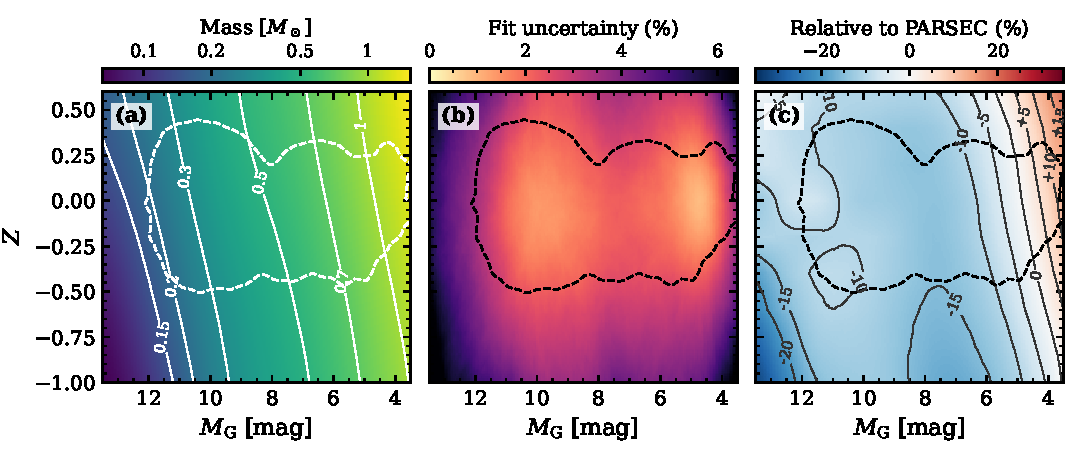
\includegraphics[width=\textwidth]{figs/mlr_surface.pdf}
\caption{Posterior MLR surface in the plane of absolute magnitude and metallicity. \emph{Panel (a):} median mass, with contours at $0.15$, $0.2$, $0.3$, $0.5$, $0.7$ and $1\,\msun$. \emph{Panel (b):} fit uncertainty, the half-width of the 16--84\% credible interval of the mass relative to the median. \emph{Panel (c):} median mass relative to PARSEC at the same $Z$, with contours every $5\%$. The dashed contour encloses 95\% of the components of the sample, placed at their $M_{\mathrm{G}}$ and at the median of the metallicity posterior of their system.}
\label{fig:mlr_surface}
\end{figure*}

\begin{figure}[t]
\centering
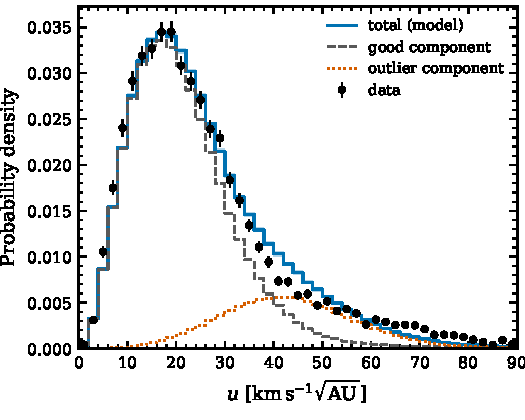
\includegraphics[width=\columnwidth]{figs/u_predictive.pdf}
\caption{Observed distribution of $u$ (points with Poisson errors) and the posterior predictive distribution of the adopted fit after the selection $u/\sigma_u>3$ (blue line: median and $68\%$ spread over $12$ posterior draws). The dashed and dotted lines show the contributions of the good and the outlier component.}
\label{fig:u_pred}
\end{figure}

% \subsection{Mass--luminosity relation at solar metallicity}
% Posterior MLR vs PARSEC at $Z=0$ (offset as a function of $M_{\mathrm{G}}$), vs \citet{Mann2019} in $M_{K_s}$;
% credible bands. Figure: MLR and ratio to PARSEC.
\begin{figure*}[t]
\centering
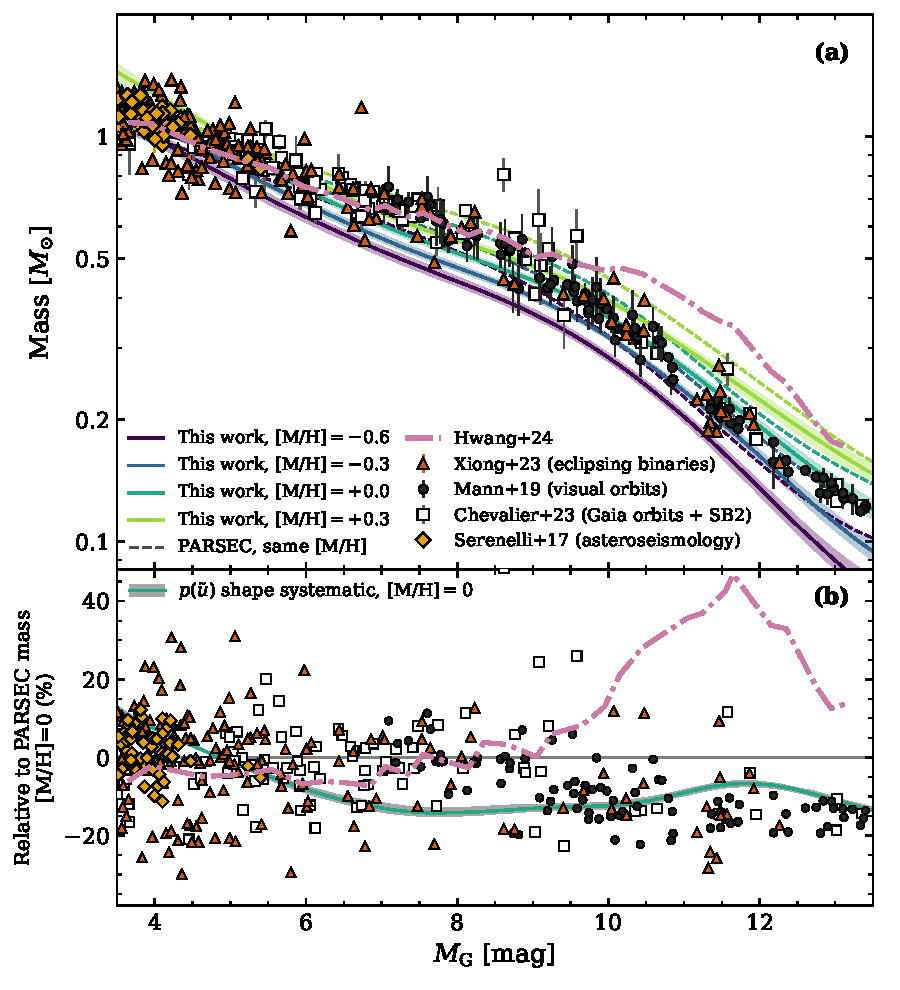
\includegraphics[width=0.7\textwidth]{figs/mlr_summary.pdf}
\caption{Dynamical MLR from this work. \emph{Panel (a):} mass as a function of $M_{\mathrm{G}}$ at $Z=-0.6,-0.3,0,+0.3$ (solid lines, shaded bands: posterior credible intervals), compared with PARSEC at the same metallicities (dashed lines), \citet{Hwang2024DynamicalMasses} (dash-dotted), and literature masses: eclipsing binaries (Xiong et al. 2023), visual orbits \citep{Mann2019}, Gaia orbits plus SB2 \citep{Chevalier2023}, and asteroseismology \citep{Serenelli2017}. \emph{Panel (b):} mass relative to PARSEC at $Z=0$. The solid line is the posterior median of this work, and the grey band is the systematic uncertainty from the shape of $p(\widetilde u)$, spanned by the MLRs obtained with eccentricity indices $\alpha_e=1.0$ and $1.5$ around the adopted $\alpha_e=1.23$ (Sect.~\ref{sec:sys_pu}). Literature points with a measured metallicity are shown only if it is within $0.15$\,dex of the solar value on their own scale; the masses of Chevalier et al. have no metallicity and are shown unfiltered.}
% TODO: add the Xiong et al. (2023) reference to refs.bib and cite it.
\label{fig:mlr_summary}
\end{figure*}

% \subsection{Metallicity dependence}
% Mass at fixed $M_{\mathrm{G}}$ as a function of $Z$; comparison with PARSEC's metallicity trend.
% Figure: MLR slices / 2D surface.
\begin{figure*}[t]
\centering
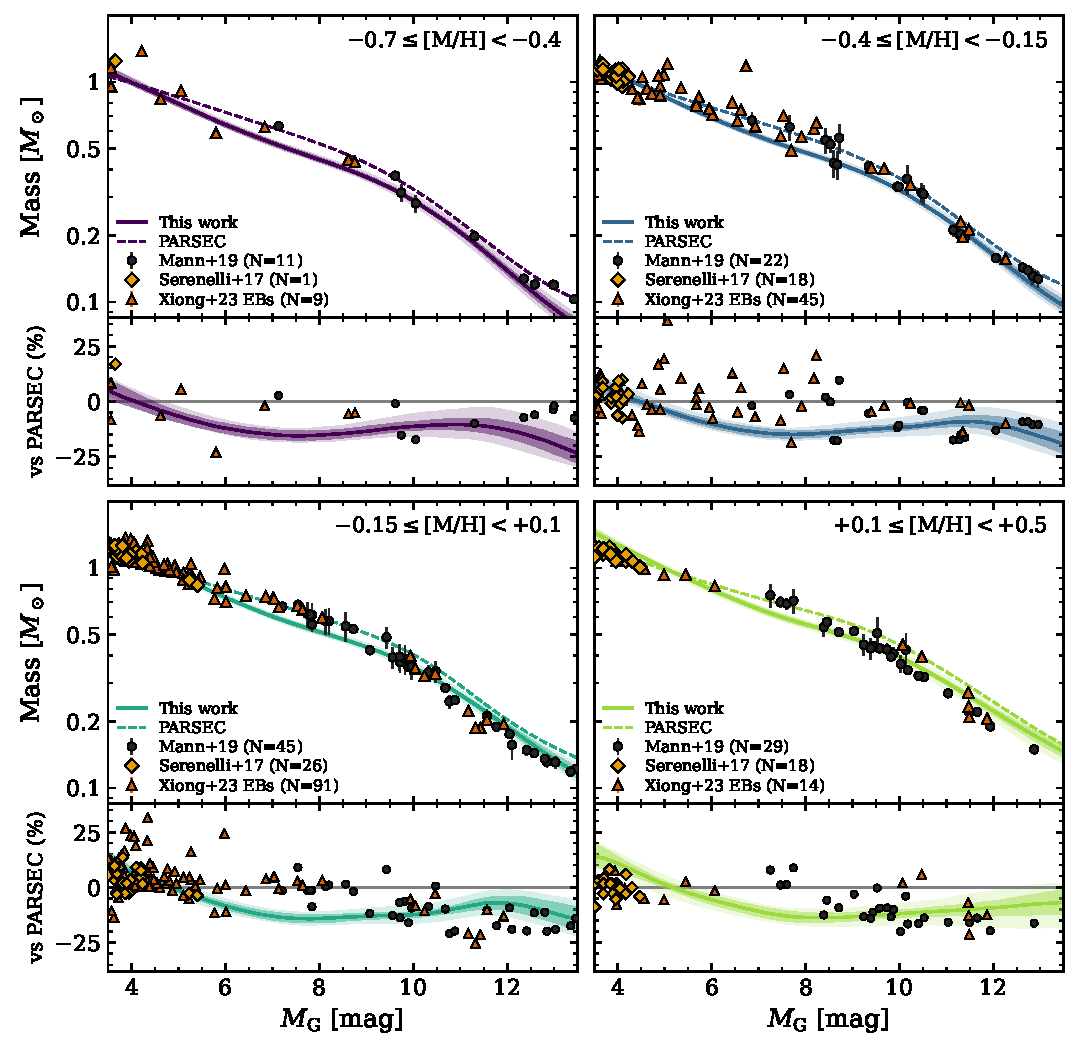
\includegraphics[width=0.85\textwidth]{figs/mlr_feh_bins.pdf}
\caption{MLR in four bins of the calibrated metallicity $Z$. The literature calibrators of Fig.~\ref{fig:mlr_summary} are not on this scale and are binned by their own measured metallicity ($[\mathrm{Fe/H}]$ for Mann et al. and Xiong et al., $[\mathrm{M/H}]$ for Serenelli et al.; sample sizes in the legends). In each bin the upper panel shows the mass and the lower panel the difference from PARSEC at the same metallicity; the solid line is the posterior MLR of this work with credible bands, and the dashed line is PARSEC.}
\label{fig:mlr_feh_bins}
\end{figure*}

% \begin{figure}[t]
% \centering
% 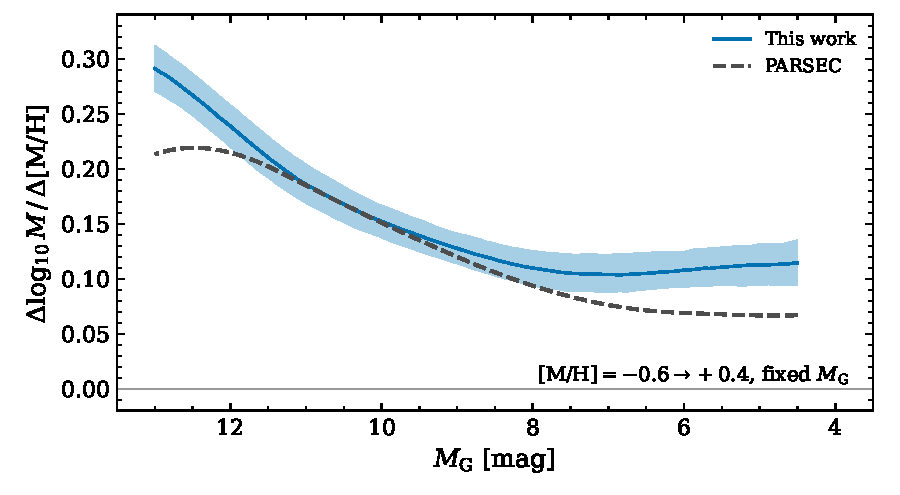
\includegraphics[width=\columnwidth]{figs/mlr_metallicity_slope.pdf}
% \caption{Metallicity sensitivity of the MLR, $\Delta\log_{10}M/\Delta Z$ between $Z=-0.6$ and $+0.4$ at fixed $M_{\mathrm{G}}$. The blue line and band show this work (posterior median and credible interval) and the dashed line shows PARSEC.}
% \label{fig:mlr_slope}
% \end{figure}
\subsection{Outlier component and goodness of fit}
The fit gives an outlier fraction before selection of $f_{\rm outlier}=0.140\pm0.004$ (posterior median and $68\%$ interval). The outlier component is more likely to pass the cut $u/\sigma_u>3$ than the good component, so the predicted fraction of outliers among the selected pairs is higher, $0.19\pm0.005$. Figure~\ref{fig:u_pred} compares the observed distribution of $u$ with the posterior predictive distribution, which is obtained by simulating for every system a replicate observation from its metallicity posterior, the MLR, the mixture of Eq.~(\ref{eq:mixture}) and its $\sigma_{u,j}$, and applying the same selection. The model reproduces the core of the distribution, where the good component dominates ($u\lesssim35\,\kmsau$). The outlier component dominates beyond $u\approx38\,\kmsau$, and there the model is not perfect: it lies slightly above the data between $40$ and $55\,\kmsau$ and below the data at $u>60\,\kmsau$, where the observed fraction of pairs is $5.7\%$ and the predicted fraction $2.8\%$. 
%The cumulative distribution of the model differs from that of the data by at most $0.025$, which is $2.3$ times the half-width of the $95\%$ Dvoretzky--Kiefer--Wolfowitz band of the data. 
The mismatch occurs where the distribution is set by the outlier component and not by the mass, because the shape of the outlier component is fixed (Sect.~\ref{sec:outlier_params}).
% TODO: stability of the mass scale with separation, distance, M_G and RUWE subsamples.


%==============================================================================
\section{Discussion}\label{sec:discussion}
% Meaning of the offset from PARSEC and Mann+19 and which stellar-model ingredients could produce it;
% metallicity dependence in context of theory; comparison with \citet{Hwang2024DynamicalMasses};
% consequences for masses of single stars from photometry; prospects (Gaia DR4, joint metallicity--dynamics model, larger XP samples).

\subsection{Compared to individual studies}
We compare our relation with four sets of mass measurements that do not rely on the dynamics of wide binaries (Figs.~\ref{fig:mlr_summary} and \ref{fig:mlr_feh_bins}). The visual orbits of nearby M dwarfs of \citet{Mann2019} give masses of the components from the orbital period and separation, to $2$--$3\%$. They are measured in the $K_s$ band, and we convert them to $M_{\mathrm{G}}$ with the PARSEC colour--magnitude relation at solar metallicity, so this conversion depends on the stellar models. Their metallicities are the $[\mathrm{Fe/H}]$ of Table~1 of that work. The detached eclipsing binaries compiled by Xiong et al. (2023) give masses of the components from the light curves and radial velocities. We take their luminosities and system $[\mathrm{Fe/H}]$, and obtain $M_{\mathrm{G}}$ from PARSEC isochrones at that metallicity, which is again model dependent, and keep only unevolved components. \citet{Chevalier2023} combine the Gaia DR3 astrometric orbits of binaries with their double-lined spectroscopic orbits to obtain the masses of both components, with the $M_{\mathrm{G}}$ from Gaia and without a metallicity. The masses of Kepler dwarfs of \citet{Serenelli2017} come from asteroseismology combined with spectroscopic parameters (the APOKASC catalogue), with the metallicity $[\mathrm{M/H}]$ of that catalogue, and we take the $M_{\mathrm{G}}$ from the Gaia DR3 magnitude and parallax without a correction for extinction. The metallicity scales of these samples are therefore different from the calibrated scale $Z$ of this work, and the comparison in a given metallicity range is approximate.
% TODO: verify the origin of the masses and metallicities of each sample against the original papers (in particular Xiong et al. 2023 and the metallicity source of Serenelli et al. 2017).

Figure~\ref{fig:mlr_summary} compares the samples with our relation at $Z=0$ and with PARSEC. Only the literature points within $0.15$\,dex of the solar metallicity on their own scale are used in the lower panel. At $M_{\mathrm{G}}<5.5$ our masses are within $5\%$ of the median masses of all samples in that range, which in turn are within $5\%$ of PARSEC. At fainter magnitudes the picture is less simple. Between $M_{\mathrm{G}}=5.5$ and $8$, where our masses are $11\%$ below PARSEC, the median masses of the visual orbits, the Gaia orbits and the eclipsing binaries are within $3\%$ of PARSEC and therefore $12$--$16\%$ above our relation. Between $M_{\mathrm{G}}=8$ and $10.5$ they are $5$--$13\%$ above our relation, and our masses are $13\%$ below PARSEC. At $M_{\mathrm{G}}>10.5$ the measured masses of all three samples lie $14$--$17\%$ below PARSEC and $2$--$8\%$ below our relation, which is $9\%$ below PARSEC. The scatter of the individual measurements around our relation is mostly $6$--$22\%$ in these bins, which includes the uncertainty of the conversion to $M_{\mathrm{G}}$ and the range of metallicities, and the samples in the individual bins are small ($6$--$38$ points). The sign of the difference from PARSEC at $M_{\mathrm{G}}>8$ agrees with the individual measurements, but at intermediate magnitudes the individual masses are on average higher than our relation. We discuss possible reasons for this in Sects.~\ref{sec:disc_isochrones} and \ref{sec:disc_mg}.

The relation of \citet{Hwang2024DynamicalMasses} follows PARSEC to within about $10\%$ at $M_{\mathrm{G}}<9$, but at $10<M_{\mathrm{G}}<12.5$ it is up to $45\%$ above PARSEC and therefore also far above the individual masses and our relation, which are below PARSEC there. Their map gives the mean mass of all stars at a position in the diagram, which includes unresolved binaries and triples, and it does not include the metallicity or the selection of the sample, and these differences probably contribute to the discrepancy.

Figure~\ref{fig:mlr_feh_bins} shows our relation in four bins of $Z$. In all bins the correction relative to PARSEC has a similar shape: it is $10$--$15\%$ below zero between $M_{\mathrm{G}}\approx6$ and $12$, and it rises towards bright magnitudes, from about $+5\%$ at $M_{\mathrm{G}}=3.5$ in the most metal-poor bin to $+15\%$ in the most metal-rich bin. The individual measurements in the same bins show the same scatter and the same trends as in Fig.~\ref{fig:mlr_summary}, but the most metal-poor bin contains only $9$ eclipsing-binary components, $11$ visual-orbit components and one asteroseismic star, which is too few to test the metallicity dependence of the relation. The sensitivity of the mass to the metallicity at a fixed magnitude is shown in Fig.~\ref{fig:mlr_slope}. The mass of our relation changes by $0.11$ and $0.10$\,dex per dex of $Z$ at $M_{\mathrm{G}}=5$ and $7$, and by $0.13$ and $0.19$\,dex per dex at $M_{\mathrm{G}}=9$ and $11$. PARSEC gives $0.07$, $0.08$, $0.12$ and $0.19$ at the same magnitudes. The metallicity dependence is therefore stronger than the PARSEC prediction by $0.03$--$0.05$\,dex per dex at $M_{\mathrm{G}}\lesssim7$, which is about twice the half-width of the $68\%$ credible band, and agrees with it at $M_{\mathrm{G}}\gtrsim9$.

\subsection{Different isochrones}\label{sec:disc_isochrones}
% TODO: comparison with other isochrones (e.g. MIST, BHAC15, Dartmouth) and the role of age and of the atmosphere and convection treatment.

\subsection{``Wrong $M_{\mathrm{G}}$, or wrong colour, or both?''}\label{sec:disc_mg}
% TODO: whether the offset from PARSEC is due to the model $M_G$, the model colour, or both; relation to the conversion of K_s and logL to M_G of the literature points.

\subsection{What can Gaia DR4 offer here?}
% TODO: prospects with Gaia DR4 (astrometric orbits and larger samples, XP spectra, better proper-motion differences, joint metallicity--dynamics model).

\subsection{Caveats and limitations}
% MLR with and without the $\mathcal A_j$ correction; size and direction of the shift.
% One consolidated list (as in Sect. 7 of the methods document): modular cut and fixed Stage-1a estimates; no $M_{\mathrm{G}}$/extinction/age
% uncertainty; fixed good and outlier shapes; only the $u/\sigma_u$ selection modelled; shared-metallicity assumption; Teff threshold; monotonicity assumption.

%==============================================================================
\section{Conclusions}\label{sec:conclusions}
We have calibrated the mass--luminosity relation of main-sequence stars in the Gaia $G$ band, over $3.5\le M_{\mathrm{G}}\le13.5$ and $-1.0\le Z\le0.6$, from the relative motion of $14\,876$ wide binaries of the \citet{ElBadry2021MillionBinaries} catalogue. The pairs are single main-sequence stars according to their Gaia XP spectra, and the metallicity of each system is the posterior of a shared value that combines the J-CaPS measurements of both components, with the relative systematics of J-CaPS calibrated from the pairs themselves and the absolute scale anchored to the Sun. The MLR is a monotone two-dimensional B-spline surface relative to PARSEC, and it is fitted with a dynamical likelihood that includes the measurement errors, an outlier component, the selection of the sample by the significance of the proper-motion difference, and the marginalisation over the metallicity posterior of each system.

Where the data are, the relation is determined to $0.9$--$3.9\%$ in mass, with a median of $2\%$. At solar metallicity our masses agree with PARSEC at $M_{\mathrm{G}}\approx5$, are higher by $7\%$ at $M_{\mathrm{G}}=4$, and are lower by $8\%$ at $M_{\mathrm{G}}=6$, $14\%$ at $M_{\mathrm{G}}=8$ and $12\%$ at $M_{\mathrm{G}}=10$, with the difference decreasing to $7\%$ at $M_{\mathrm{G}}=12$. The mass depends more strongly on metallicity than PARSEC predicts at $M_{\mathrm{G}}\lesssim7$, by $0.03$--$0.05$\,dex per dex, and agrees with it at $M_{\mathrm{G}}\gtrsim9$. The adopted shape of $p(\widetilde u)$ has the largest known systematic effect, of $1$--$1.6\%$ in mass, and it is smaller than the statistical uncertainty. The model describes the core of the observed distribution of $u$, but it underpredicts the tail at $u>60\,\kmsau$ because the shape of the outlier component is fixed, and we have not yet quantified the effect on the MLR. Individual mass measurements from visual orbits, Gaia orbits, eclipsing binaries and asteroseismology agree with our relation at $M_{\mathrm{G}}<5.5$ and have the same sign of the difference from PARSEC at $M_{\mathrm{G}}>10.5$, but at $5.5<M_{\mathrm{G}}<10.5$ their masses are $5$--$16\%$ higher than ours. Understanding this difference is the main open question of this work. The relation can be improved with the larger and more precise astrometric samples and spectra of future Gaia data releases, which will also allow the metallicity and the dynamics to be modelled jointly.

\begin{acknowledgements}
% Funding, Gaia acknowledgement, software (NumPyro, JAX, astropy, matplotlib).
\end{acknowledgements}

\bibliographystyle{aa}
\bibliography{refs}

\begin{appendix}

\section{System metallicities}
% Relative calibration offset and scatter; population metallicity distribution; comparison of shared-$Z$ posteriors
% with raw per-star values.

\section{Full model specification}\label{app:model}
\paragraph{Monotone parametrisation.} The coefficient grid $\Theta$ is generated from unconstrained variables, so that Eq.~(\ref{eq:coefficient-order}) holds for every draw. With $\softplus(t)=\ln(1+e^t)$, $\sigmoid(t)=(1+e^{-t})^{-1}$ and positive scales $\lambda_x,\lambda_Z$, the first row and column are
\begin{align}
 \Theta_{11}&=c_0,\\
 \Theta_{1h}&=\Theta_{1,h-1}+\lambda_Z\softplus(a_h),\quad h=2,\ldots,4,\\
 \Theta_{i1}&=\Theta_{i-1,1}-\lambda_x\softplus(b_i),\quad i=2,\ldots,8,
\end{align}
and the interior points, visited in increasing $i+h$, lie between their two predecessors,
\begin{align}
 \Theta_{ih}&=L_{ih}+(U_{ih}-L_{ih})\sigmoid(r_{ih}),\\
 L_{ih}&=\Theta_{i,h-1},\quad U_{ih}=\Theta_{i-1,h}.
\end{align}
If the previously constructed points obey both orders, then $L_{ih}\le\Theta_{i-1,h-1}\le U_{ih}$, so the interval is non-empty and the new point satisfies both inequalities; induction over $i+h$ gives Eq.~(\ref{eq:coefficient-order}) for the complete grid. The derivative of a B-spline surface is a sum of non-negative basis functions weighted by differences of adjacent coefficients, so the coefficient orders fix the signs of $\partial g/\partial x$ and $\partial g/\partial Z$ everywhere in the domain.

\paragraph{Priors.} The parameters and priors of the three stages are listed in Table~\ref{tab:priors}. The coordinates $(c_0,a_h,b_i,r_{ih},\log\lambda_x,\log\lambda_Z,f_{\rm outlier})$ give $35$ free parameters. Here $\Pi_{11}=0.00703$, and $\lambda_{x,\rm ref}=0.18624$ and $\lambda_{Z,\rm ref}=0.13078$\,dex are the mean coefficient increments of the PARSEC surface. Three further factors act on the surface rather than on a sampled coordinate. The shrinkage $\log\pi_{\rm shrink}=-\sum_{ih}D_{ih}^2/(2\tau_D^2)$ pulls the correction to zero. The smoothness term $\log\pi_{\rm smooth}$ is a Gaussian penalty on the second differences of $D$ along $x$ and along $Z$ and on its mixed difference, each normalised by the spacing of the Greville abscissae of the spline and with width $\tau_x=\tau_Z=\tau_{xZ}=0.05$\,dex \citep{EilersMarx1996PSplines}. The solar anchor is a Gaussian on $g(M_{\mathrm{G},\odot},0)$ with mean $0$ and width $0.01/\ln10\approx0.0043$\,dex, which fixes the absolute mass scale to $1\%$ at the solar magnitude and metallicity without forcing the correction to vanish there. None of these terms enforces the signs of slopes or curvature. Figure~\ref{fig:prior_pred} shows the prior on the sampled coordinates projected onto the mass--$M_{\mathrm{G}}$ plane. It is broad compared with the posterior, with a spread of more than an order of magnitude in mass at faint magnitudes, so the posterior is determined by the data and not by the prior.

\begin{table*}[ht]
\centering
\caption{Parameters and priors. Normal distributions are given as location and standard deviation.}
\label{tab:priors}
\small
\begin{tabular}{@{}llll@{}}
\toprule
Stage & Quantity & Prior & Role \\
\midrule
1a & $(b,s_z,\nu)$ & maximum likelihood & relative calibration; fixed in 1b \\
1b & $\delta_z$ & fixed to $0$ (solar anchor) & absolute zero point \\
1b & $\bm\omega$ & Dirichlet$(1,\ldots,1)$ & population weights \\
2 & $c_0$ & $\Normal(\Pi_{11},0.10)$\,dex & first coefficient \\
2 & $a_h,b_i,r_{ih}$ & $\Normal(0,1)$ & monotone coordinates \\
2 & $\log\lambda_x$ & $\Normal(\ln\lambda_{x,\rm ref},0.7)$ & increment scale in $x$ \\
2 & $\log\lambda_Z$ & $\Normal(\ln\lambda_{Z,\rm ref},0.7)$ & increment scale in $Z$ \\
2 & $f_{\rm outlier}$ & Beta$(3,12)$ & outlier fraction before selection \\
2 & $D_{ih}=\Theta_{ih}-\Pi_{ih}$ & $\Normal(0,\tau_D=0.10)$\,dex & shrinkage to PARSEC \\
2 & second differences of $D$ & $\Normal(0,\tau=0.05)$\,dex & smoothness in $x$, $Z$ and mixed \\
2 & $g(M_{\mathrm{G},\odot},0)$ & $\Normal(0,0.01/\ln10)$\,dex & solar mass anchor ($1\,\msun\pm1\%$) \\
\bottomrule
\end{tabular}
\end{table*}

\begin{figure*}[t]
\centering
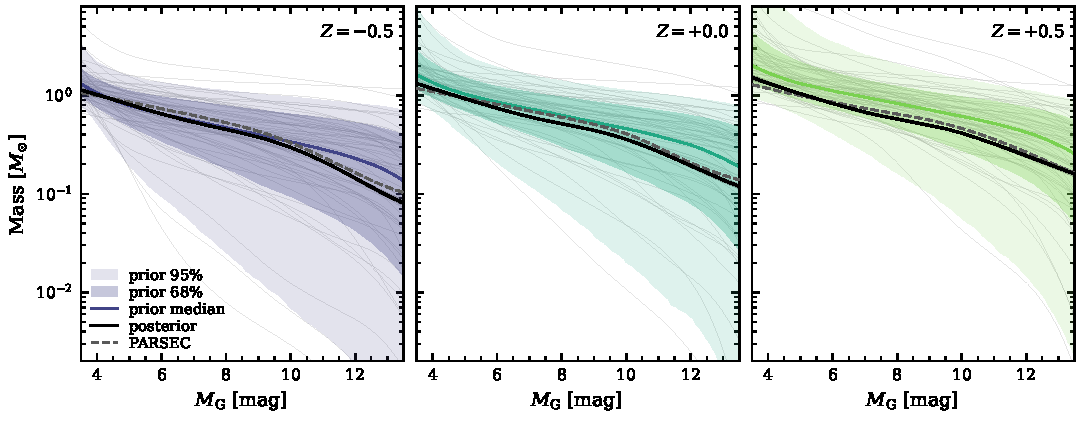
\includegraphics[width=\textwidth]{figs/prior_predictive.pdf}
\caption{Prior of the MLR surface projected onto the mass--$M_{\mathrm{G}}$ plane at three metallicities. The shaded bands show the $68\%$ and $95\%$ ranges of $4\,000$ draws from the priors on the sampled coordinates of Table~\ref{tab:priors}, the coloured line is their median, and a subset of the draws is drawn in grey. The shrinkage, smoothness and solar-anchor terms act on the derived surface and are not included. The black line and band are the median and $68\%$ interval of the posterior, and the dashed line is PARSEC at the same metallicity. Every prior draw is monotone in $M_{\mathrm{G}}$ and $Z$ by construction.}
\label{fig:prior_pred}
\end{figure*}


\section{Corner plots, convergence diagnostics, binned MLR values}
% Corner plots, convergence diagnostics, binned MLR values.


\section{Mock-data validation}\label{app:mock}
% Recovery of an input MLR from simulated wide binaries with and without the selection cut; coverage of credible intervals.


\section{Systematic checks}\label{sec:systematics}
\subsection{Shape of $p(\widetilde u)$}\label{sec:sys_pu}
The statistic $\widetilde u$ depends only on the eccentricity, the orbital phase and the orientation of a pair. The semi-major axis and the distance enter only through the selection of the sample, which acts on the observed projected separation $s_{\rm proj}$ and the distance $d$. The distribution needed by the likelihood is therefore
\begin{equation}
 p(\widetilde u\mid\text{sample})=\int p(\widetilde u\mid s_{\rm proj},d)\,p_{\rm sample}(s_{\rm proj},d)\dd s_{\rm proj}\dd d .
\end{equation}
We simulate $4\times10^6$ Keplerian orbits with semi-major axes log-uniform between $10$ and $10^5$\,au, distances log-uniform between $5$ and $1000$\,pc, mean anomalies uniform in $[0,2\pi)$, isotropic orientations, and eccentricities drawn from $p(e)=(1+\alpha_e)e^{\alpha_e}$. Kepler's equation is solved for the true anomaly, and the projected separation and projected relative velocity give $\widetilde u$ for each orbit. Each simulated pair inside the range of the sample in $s_{\rm proj}$ and $d$ receives the weight $w=H_{\rm sample}/H_{\rm sim}$, the ratio of the normalised two-dimensional histograms of the sample and of the simulation in $24$ bins of $\log s_{\rm proj}$ and $18$ bins of $\log d$. Because the angular separation is $\theta=s_{\rm proj}/d$, the weights also reproduce the angular-resolution limit of the catalogue, and an additional cut $\theta>1.5''$ or $3''$ leaves the fitted constants unchanged. Eq.~(\ref{eq:good}) is fitted by least squares to the weighted histogram of $\widetilde u$ in $100$ bins on $[0,40]$. All values of $\alpha_e$ use the same random numbers for the phases, orientations and eccentricity quantiles, so that the differences between the shapes contain no simulation noise.

\citet{Hwang2022Eccentricity} describe the power-law index as a function of $w=\log_{10}(s_{\rm proj}/\mathrm{au})$ by $\alpha(w)=1.25\tanh[(w-1.87)/0.88]+0.12$. Evaluated at the projected separations of our pairs, it ranges from $1.04$ to $1.34$ (5th to 95th percentile), because only $1\%$ of the pairs have $s_{\rm proj}<300$\,au. Drawing one eccentricity for each pair from its $p(e\mid\alpha(w))$ and fitting a single power law to the pooled values by maximum likelihood gives $\alpha_e=1.23\pm0.02$, which we adopt. A simulation with the separation-dependent index applied to each orbit gives a shape with the same median of $\widetilde u$ to within $0.02$. The fitted constants are listed in Table~\ref{tab:pu}.

\begin{table}
\caption{Constants of Eq.~(\ref{eq:good}) for three eccentricity indices.}
\label{tab:pu}
\centering
\begin{tabular}{ccccc}
\toprule
$\alpha_e$ & $B$ & $u_c$ & $C$ & median $\widetilde u$ \\
\midrule
1.0 & $2.2943\times10^{-3}$ & 36.2851 & 3.5567 & 16.36 \\
1.23 & $2.5050\times10^{-3}$ & 37.2461 & 2.4500 & 16.08 \\
1.5 & $2.6522\times10^{-3}$ & 37.9042 & 1.7151 & 15.82 \\
\bottomrule
\end{tabular}
\tablefoot{The adopted shape is $\alpha_e=1.23$. Medians in $\kmsau$.}
\end{table}

The shape of $p(\widetilde u)$ is fixed by the orbital elements of the population, and of these only the eccentricity distribution is not determined by the sample itself: the phases and orientations are random, and the dependence on the separation and distance distributions is removed by the weighting of Appendix~\ref{app:pu}. A more eccentric population spends a larger fraction of each orbit near apocentre, at large separation and low speed, so $p(\widetilde u)$ moves to lower values and the masses inferred at fixed $u$ increase. We repeat the full inference, including the per-pair likelihood tables, with the shapes for $\alpha_e=1.0$ and $1.5$ (Table~\ref{tab:pu}). The lower value is the thermal distribution. It allows for the bias of the measured index towards higher values that \citet{Hwang2022Eccentricity} attribute to their cut on the significance of the proper-motion difference, which at separations above $10^{3.5}$\,au they estimate at about $0.1$, and for the extrapolation from their sample within 200\,pc to ours within 1\,kpc. The upper value allows for unresolved companions, which randomise the measured velocity directions and bias the index towards the thermal value.

At $Z=0$, $\alpha_e=1.0$ lowers the masses by $0.4$--$1.0\%$ and $\alpha_e=1.5$ raises them by $0.5$--$1.6\%$ over $5\le M_{\mathrm{G}}\le13$, with the largest change at $M_{\mathrm{G}}\approx8$ (Fig.~\ref{fig:mlr_summary}b). At $M_{\mathrm{G}}=4$ both changes are below $0.3\%$. The metallicity slices $Z=-0.6$ and $+0.3$ change by the same amounts to within $0.6\%$, so the metallicity dependence of the MLR is not affected. At every $M_{\mathrm{G}}$ the change is smaller than the half-width of the 68\% credible interval, which is $1$--$2\%$ at $5\le M_{\mathrm{G}}\le10$ and rises to $5\%$ at $M_{\mathrm{G}}=13$. The outlier fraction and the convergence of the sampler are the same for the three shapes.

\subsection{Outlier model parameters}\label{sec:outlier_params}
% TODO: choice of the outlier model (mean and width of the Gaussian, its truncation, mass dependence) and its effect on the MLR; the
% model underpredicts the tail at u > 60 km/s sqrt(AU) (Fig. 4).
% Further checks to be added: Teff threshold, metallicity anchor, priors on the correction, RUWE and separation subsamples.

\end{appendix}

\end{document}
